\documentclass[a4paper, portrait,11pt]{article}
\usepackage{polski}
\usepackage[utf8]{inputenc}
\usepackage{amsmath}
\usepackage{graphicx}
\usepackage{hyperref}
\usepackage{listings}
\usepackage{subcaption}
\usepackage{numprint}
\usepackage[justification=centering]{caption}
\usepackage[margin=0.5in]{geometry}
\npdecimalsign{.}
\nprounddigits{3}

\title{\textbf{Zadanie 3 - Inteligentna Analiza Danych}}
\author{
  Adam Zambrzycki\\
  \texttt{Nr indeksu: 216933}
  \and
  Konrad Stępniak\\
  \texttt{Nr indeksu: 216892}
}

\begin{document}
\maketitle
  \begin{tabular}{ll}
    \textbf{Kierunek} & Informatyka\\
    \textbf{Rok akademicki} & {2018/19} \\
    \textbf{Semestr} & {4} \\
    \textbf{Grupa dziekańska}& {2} \\ \\ \\
  \end{tabular}

Symbol $\alpha$ będzie oznaczał współczynnik nauki, a $K$ liczbę centrów.

\section{Osobna nauka warstw - Aproksymacja}
Do nauki wykorzystano następujące parametry: $\alpha=0.05$, liczba iteracji $= 20000$.
\subsection{Podzadanie 1}

\begin{figure}[!htb]
  \begin{minipage}{0.33\textwidth}
    \centering
    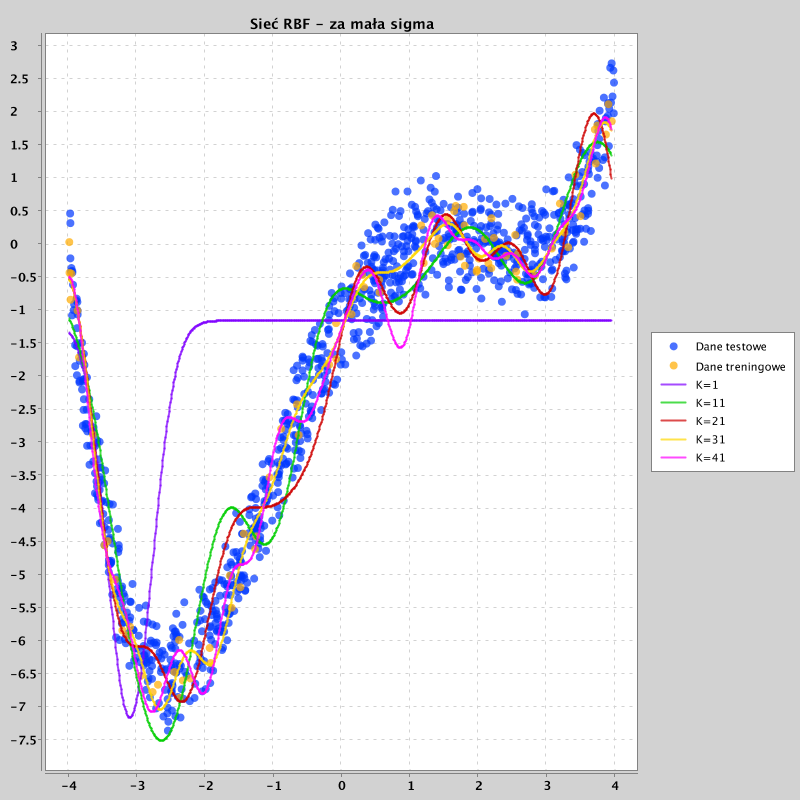
\includegraphics[width=1\linewidth]{../data/approximation3/1/small.png}
    \caption{Za mała sigma}
  \end{minipage}
  \begin{minipage}{0.33\textwidth}
    \centering
    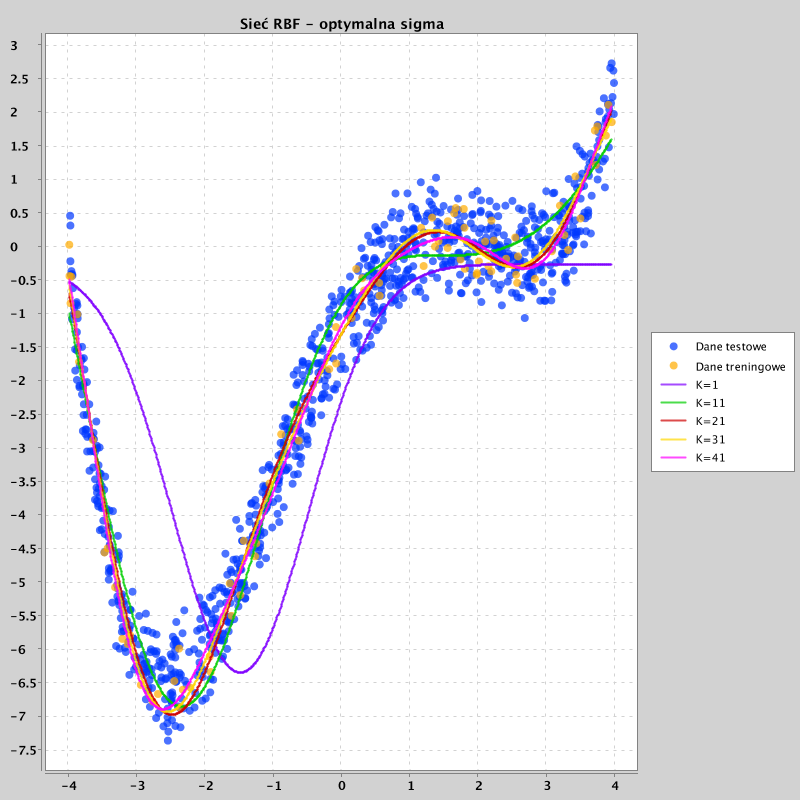
\includegraphics[width=1\linewidth]{../data/approximation3/1/optimal.png}
    \caption{Optymalna sigma}
  \end{minipage}
  \begin{minipage}{0.33\textwidth}
    \centering
    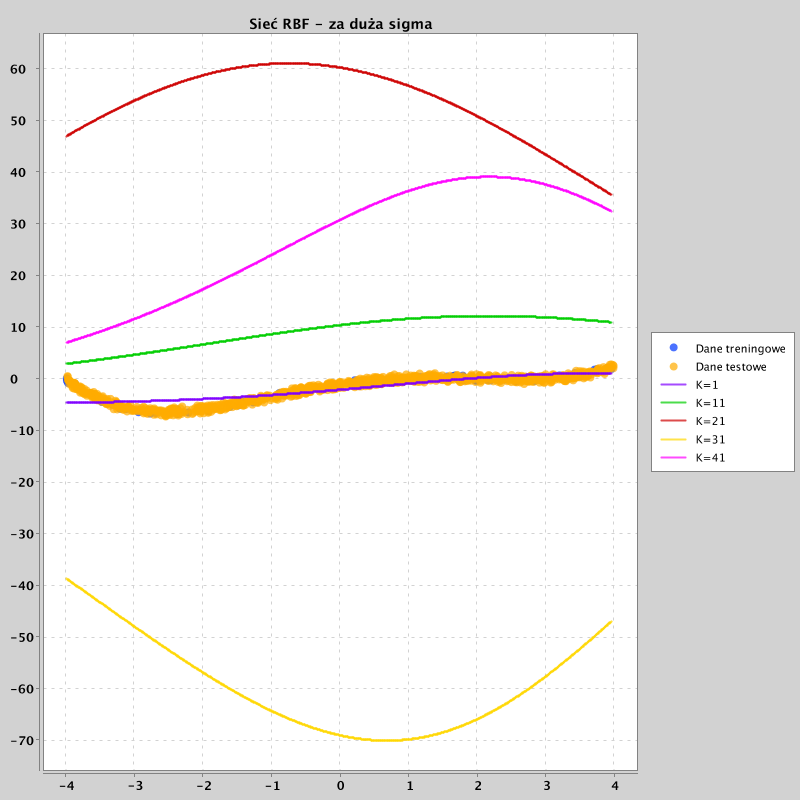
\includegraphics[width=1\linewidth]{../data/approximation3/1/big.png}
    \caption{Za duża sigma}
  \end{minipage}\hfill
\end{figure}

\subsection{Podzadanie 2}

Czerwone linie reprezentują funkcje pojedynczych neuronów.
\begin{figure}[!htb]
  \begin{minipage}{0.33\textwidth}
    \centering
    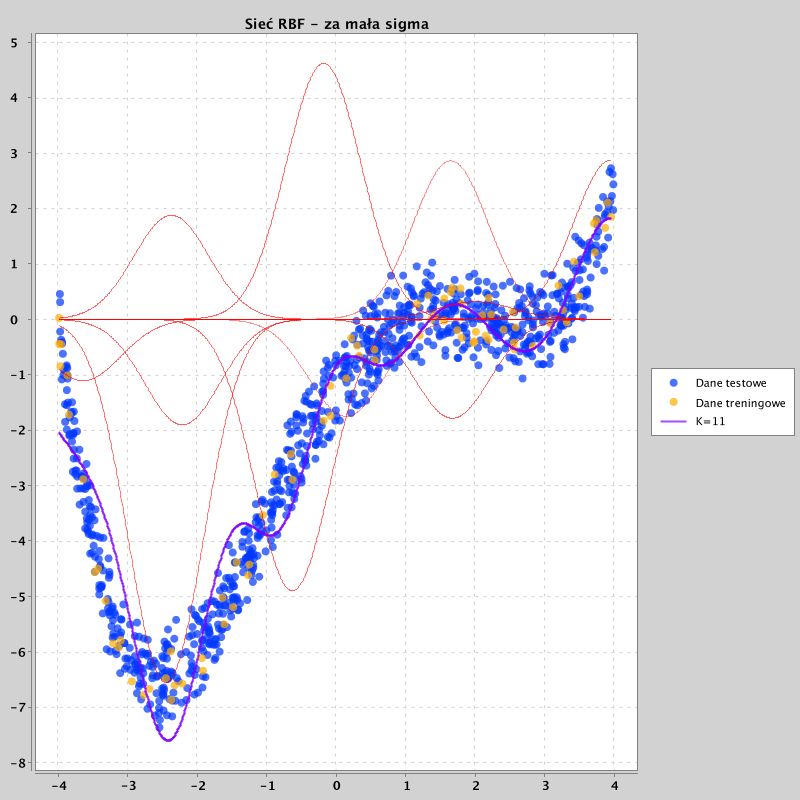
\includegraphics[width=1\linewidth]{../data/approximation3/2/small.png}
    \caption{Za mała sigma}
  \end{minipage}
  \begin{minipage}{0.33\textwidth}
    \centering
    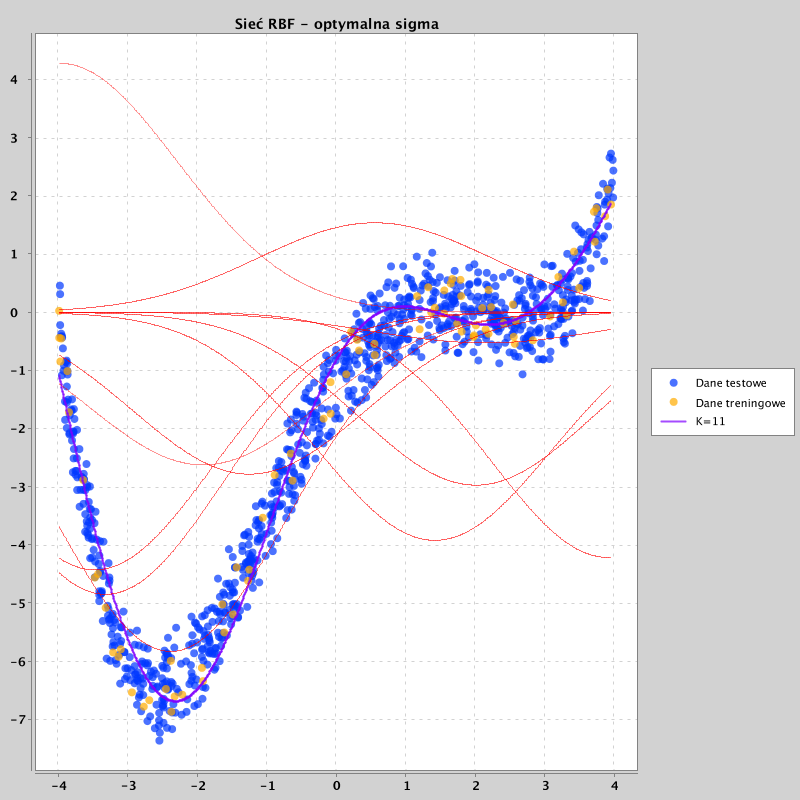
\includegraphics[width=1\linewidth]{../data/approximation3/2/optimal.png}
    \caption{Optymalna sigma}
  \end{minipage}
  \begin{minipage}{0.33\textwidth}
    \centering
    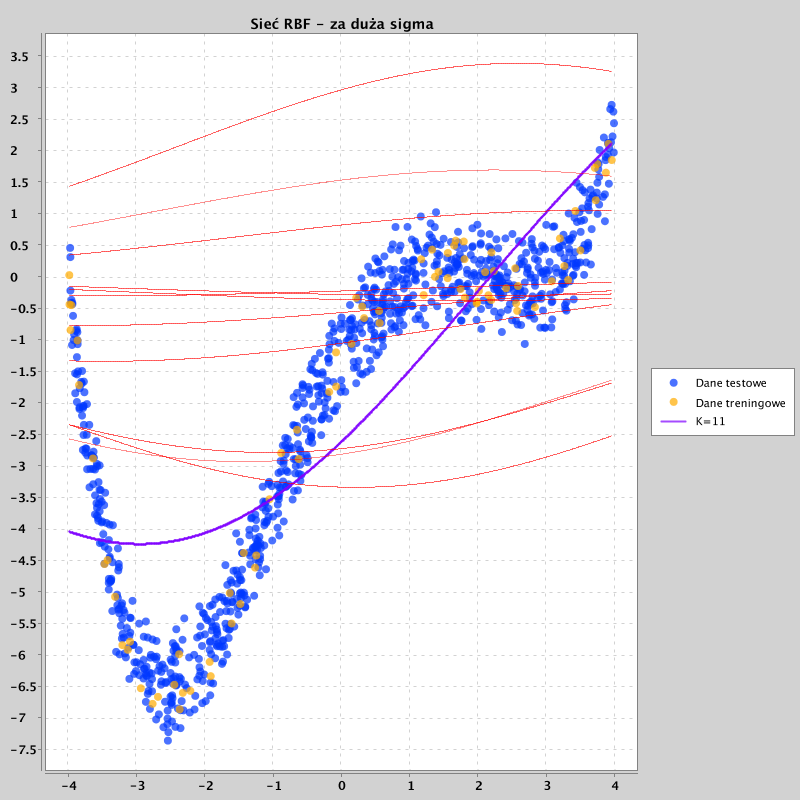
\includegraphics[width=1\linewidth]{../data/approximation3/2/big.png}
    \caption{Za duża sigma}
  \end{minipage}\hfill
\end{figure}


\subsection{Podzadanie 3}
Symbole $\epsilon_a$, $\epsilon_b$ oznaczają błędy średniokwadratowe odpowiednio dla zbioru treningowego i testowego. 
Symbol $\sigma$ w Tabeli \ref{table:approx3} oznacza odchylenie standardowe.
\begin{table}[h!]
  \caption{\label{table:approx3}Błąd średniokwadratowy oraz odchylenie dla zbioru treningowego i testowego dla 100 prób nauki}
  \centering
  \begin{tabular}{|l|n{1}{3}|n{1}{3}|n{1}{3}|n{1}{3}|}
    \hline
    \textbf{K} & \textbf{$avg(\epsilon_a)$} & \textbf{$\sigma(\epsilon_a)$} & \textbf{$avg(\epsilon_b)$} & \textbf{$\sigma(\epsilon_b)$}\\
    \hline
    1 & 2.2487527537653222 & 0.6261100919193574 & 1.955473836265807 & 0.5621825986540743 \\
    6 & 0.28568563944924996 & 0.2858213621279681 & 0.2522575453670399 & 0.19566409363294007 \\
    11 & 0.15128659994761162 & 0.11688975023198557 & 0.1680474127628648 & 0.07502859293396406 \\
    16 & 0.07765026065094292 & 0.02498215607290317 & 0.11514668896463105 & 0.01780284915773643 \\
    21 & 0.06057939963788164 & 0.016323733595582136 & 0.10661257959927159 & 0.009578394200630884 \\
    26 & 0.05789604352158822 & 0.009466525235758683 & 0.10751656209053062 & 0.007975489839156847 \\
    31 & 0.0515018661618608 & 0.005740971340396712 & 0.10206851520703669 & 0.005089507447365943 \\
    36 & 0.04704336994595712 & 0.0033461785075818125 & 0.09778242471482931 & 0.0032371893229406067 \\
    41 & 0.04561073842684816 & 0.0031295651169926855 & 0.09715678881154301 & 0.003091645909513203 \\
    \hline
  \end{tabular}
\end{table}

\subsection{Podzadanie 4}
\begin{figure}[!htb]
  \centering
  \begin{minipage}{0.5\textwidth}
    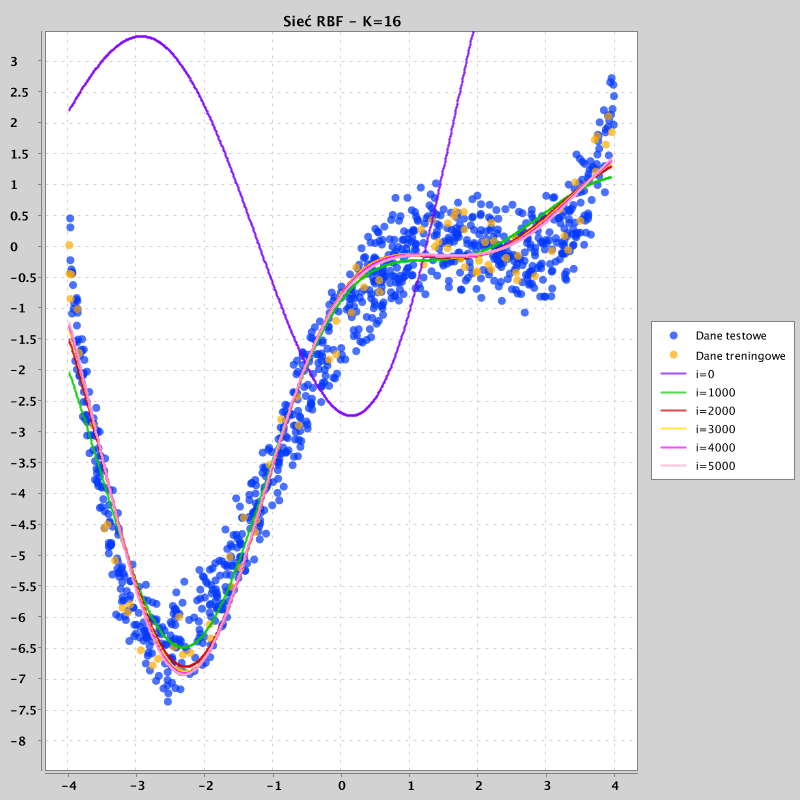
\includegraphics[width=1\linewidth]{../data/approximation3/4/chart.png}
    \caption{Zmiana funkcji sieci w różnych momentach}
  \end{minipage}\hfill
\end{figure}


\end{document}